%! Author = yuliu
%! Date = 10/10/2024

% Options for packages loaded elsewhere
\PassOptionsToPackage{unicode}{hyperref}
\PassOptionsToPackage{hyphens}{url}
\documentclass[letterpaper, 11pt]{article}
% Set 1-inch margins and 0.5-inch header and footer
\usepackage[margin=1in, headheight=0.5in, footskip=0.5in]{geometry}
\usepackage{xcolor}
\usepackage{amsmath,amssymb}
\setcounter{secnumdepth}{-\maxdimen} % remove section numbering
\usepackage{iftex}
\ifPDFTeX
\usepackage[T1]{fontenc}
\usepackage[utf8]{inputenc}
\usepackage{textcomp} % provide euro and other symbols
\else % if luatex or xetex
\usepackage{unicode-math} % this also loads fontspec
\defaultfontfeatures{Scale=MatchLowercase}
\defaultfontfeatures[\rmfamily]{Ligatures=TeX,Scale=1}
\fi
\usepackage{lmodern}
\ifPDFTeX\else
% xetex/luatex font selection
\fi
% Use upquote if available, for straight quotes in verbatim environments
\IfFileExists{upquote.sty}{\usepackage{upquote}}{}
\IfFileExists{microtype.sty}{% use microtype if available
\usepackage[]{microtype}
\UseMicrotypeSet[protrusion]{basicmath} % disable protrusion for tt fonts
}{}
\makeatletter
\@ifundefined{KOMAClassName}{% if non-KOMA class
\IfFileExists{parskip.sty}{%
\usepackage{parskip}
}{% else
\setlength{\parindent}{0pt}
\setlength{\parskip}{6pt plus 2pt minus 1pt}}
}{% if KOMA class
\KOMAoptions{parskip=half}}
\makeatother
\usepackage{longtable,booktabs,array}
\usepackage{calc} % for calculating minipage widths
% Correct order of tables after \paragraph or \subparagraph
\usepackage{etoolbox}
\makeatletter
\patchcmd\longtable{\par}{\if@noskipsec\mbox{}\fi\par}{}{}
\makeatother
% Allow footnotes in longtable head/foot
\IfFileExists{footnotehyper.sty}{\usepackage{footnotehyper}}{\usepackage{footnote}}
\makesavenoteenv{longtable}
\usepackage{graphicx}
\makeatletter
\newsavebox\pandoc@box
\newcommand*\pandocbounded[1]{% scales image to fit in text height/width
\sbox\pandoc@box{#1}%
\Gscale@div\@tempa{\textheight}{\dimexpr\ht\pandoc@box+\dp\pandoc@box\relax}%
\Gscale@div\@tempb{\linewidth}{\wd\pandoc@box}%
\ifdim\@tempb\p@<\@tempa\p@\let\@tempa\@tempb\fi% select the smaller of both
\ifdim\@tempa\p@<\p@\scalebox{\@tempa}{\usebox\pandoc@box}%
\else\usebox{\pandoc@box}%
\fi%
}
% Set default figure placement to htbp
\def\fps@figure{htbp}
\makeatother
\ifLuaTeX
\usepackage{luacolor}
\usepackage[soul]{lua-ul}
\else
\usepackage{soul}
\fi
\setlength{\emergencystretch}{3em} % prevent overfull lines
\providecommand{\tightlist}{%
\setlength{\itemsep}{0pt}\setlength{\parskip}{0pt}}
\usepackage{bookmark}
\IfFileExists{xurl.sty}{\usepackage{xurl}}{} % add URL line breaks if available
\urlstyle{same}
\hypersetup{
hidelinks,
pdfcreator={LaTeX via pandoc}}

\usepackage{adjustbox}

%%%%%%%%%%%%%%%%%%%%%%%%%%%%%%%%%%%% Customized Commands %%%%%%%%%%%%%%%%%%%%%%%%%%%%%%%%%%%%
\usepackage{color}

% for strikethrough \st
\usepackage{soul}

\usepackage{blindtext}
\usepackage{hyperref}
\usepackage{crossreftools}

\usepackage{xstring}
\usepackage{xparse}

\usepackage{xstring} % Required for \StrBefore and \StrBehind
\usepackage{hyperref} % Required for \nameref functionality
\usepackage{etoolbox} % Required for \protected@edef

\usepackage[final]{pdfpages} % include pdf files
\usepackage{graphicx} % Required for \graphicspath

% Set the default path for figures and PDFs
\graphicspath{{media/}{exhibits/}{photocopies/}{forms/}}

\newcommand{\red}[1]{{\color{red}#1}}
\newcommand{\blue}[1]{{\color{blue}#1}}
\newcommand{\green}[1]{{\color{green}#1}}

% Placeholder for name
\newcommand{\myname}{{\color{red}First Last~}}

% Define \exhibittext to save exhibit text and number, with a conditional comma before #3 if #3 is not empty
\newcommand{\exhibittext}[3]{%
  \expandafter\gdef\csname #1text\endcsname{%
    Exhibit #2%
    \ifx\relax#3\relax % Check if #3 is empty
      % Do nothing if #3 is empty
    \else
      ,~#3 % Add a comma and #3 if #3 is not empty
    \fi
  }%
  \expandafter\gdef\csname #1num\endcsname{#2} % Save the exhibit number separately
  \textcolor{blue}{\it \textbf{(Exhibit #2%
    \ifx\relax#3\relax % Same check for display in blue
      % Do nothing if #3 is empty
      )
    \else
      , #3) % Add a comma and #3 if #3 is not empty
    \fi
  }}%
  \label{#1} % Define a label
}


% Update \labelexhibit to create a new exhibit text combining old text and new text, and store with new label
\newcommand{\labelexhibit}[3]{%
  \ifcsname #3text\endcsname % Check if the new exhibit label already has text
    \expandafter\edef\csname #3text\endcsname{Exhibit \csname #1num\endcsname~#2} % Append new text with a separator
    % \expandafter\gdef\csname #3text\endcsname{~#2}
    \textcolor{blue}{{\textbf{Exhibit \csname #1num\endcsname}~#2}}
  \else
    \expandafter\gdef\csname #3text\endcsname{Exhibit #1~#2} % Define new text if not previously defined
    \textcolor{blue}{\textbf{Exhibit #1}~#2}
  \fi
  \label{#3} % Create a label for referencing with the new label
}

% Update \labelexhibit to create a new exhibit text combining old text and new text, and store with new label
\newcommand{\labelexhibitsub}[3]{%
  \ifcsname #3text\endcsname % Check if the new exhibit label already has text
    \expandafter\edef\csname #3text\endcsname{Exhibit \csname #1num\endcsname~#2} % Append new text with a separator
    % \expandafter\gdef\csname #3text\endcsname{~#2}
    \textcolor{blue}{\textbf{\hspace{3.6em}\csname #1num\endcsname}~#2}
  \else
    \expandafter\gdef\csname #3text\endcsname{Exhibit #1~#2} % Define new text if not previously defined
    \textcolor{blue}{\textbf{\hspace{3.6em}#1}~#2}
  \fi
  \label{#3} % Create a label for referencing with the new label
}

% Command to retrieve and display exhibit text split across two lines,
% removing any content after the first comma in \exhibitText
\newcommand{\refexhibitlabel}[1]{%
  \ifcsname #1text\endcsname % Check if the exhibit text exists
    \edef\fulltext{\csname #1text\endcsname} % Capture the saved text
    \StrBefore{\fulltext}{~}[\exhibitNumber] % Extract text before ~
    \StrBehind{\fulltext}{~}[\exhibitText]   % Extract text after ~
    \begin{center}
    \textcolor{blue}{\fontsize{20}{0}\selectfont\textbf{\exhibitNumber}} \vspace{3em} \par \textcolor{blue}{\fontsize{15}{0}\selectfont\exhibitText}
    \vspace{2em}
    \end{center}
  \else
    \textcolor{red}{Undefined exhibit: #1} % Error message if exhibit not found
  \fi
}

% Command to retrieve and display exhibit text split across two lines,
% removing any content after the first comma in \exhibitText
\newcommand{\refexhibitsublabel}[1]{%
  \ifcsname #1text\endcsname % Check if the exhibit text exists
    \edef\fulltext{\csname #1text\endcsname} % Capture the saved text
    \StrBefore{\fulltext}{~}[\exhibitNumber] % Extract text before ~
    \StrBehind{\fulltext}{~}[\exhibitText]   % Extract text after ~
    % \begin{center}
    \vspace{1em}
    \textcolor{blue}{\fontsize{15}{0}\selectfont\textbf{\exhibitNumber}}\hspace{1em}\textcolor{blue}{\fontsize{12}{0}\selectfont\exhibitText}
    % \end{center}
  \else
    \textcolor{red}{Undefined exhibit: #1} % Error message if exhibit not found
  \fi
}

% Command to retrieve and display exhibit text split across two lines,
% removing any content after the first comma in \exhibitText
\newcommand{\refexhibitaddsublabel}[3]{%
  \ifcsname #1text\endcsname % Check if the exhibit text exists
    \edef\fulltext{\csname #1text\endcsname} % Capture the saved text
    \StrBefore{\fulltext}{~}[\exhibitNumber] % Extract text before ~
    \StrBehind{\fulltext}{~}[\exhibitText]   % Extract text after ~
    % \begin{center}
    \vspace{1em}
    \textcolor{blue}{\fontsize{15}{0}\selectfont\textbf{\exhibitNumber-#2}}\hspace{1em}\textcolor{blue}{\fontsize{12}{0}\selectfont#3}
    % \end{center}
  \else
    \textcolor{red}{Undefined exhibit: #1} % Error message if exhibit not found
  \fi
}



\newcommand{\refexhibit}[1]{\textcolor{blue}{\it \textbf{{\csname #1text\endcsname}}}}
\newcommand{\refexhibitnum}[1]{\textcolor{blue}{\it \textbf{(Exhibit {\csname #1num\endcsname})}}}%

%%%%%%%%%%%%%%%%%%%%%%%%%%%%%%%%%%%% Customized Commands %%%%%%%%%%%%%%%%%%%%%%%%%%%%%%%%%%%%

\author{}
\date{}

\begin{document}
% no page numbers
\thispagestyle{empty}
% cover letter
\begin{center}
    \section{} % create space
    \section{\fontsize{20}{0}\selectfont Cover Letter}
    \section{} % create space
\end{center}

\section{Subject: National Interest Waiver Petition}\label{subject-national-interest-waiver-petition}

Dear Sir/Madam,

I am writing to respectfully submit my petition for a \textbf{National Interest Waiver (NIW)} under the employment-based, second preference (EB-2) immigrant visa category.

Included in this petition package are the following documents, which collectively attest to the national interest of my work and my qualifications for a National Interest Waiver:

\begin{enumerate}
\def\labelenumi{\arabic{enumi}.}
\item
  \textbf{The check (\$715) payable to the U.S. Department of Homeland
  Security for I-140 Application fee}
\item
  \textbf{The check (\$2,805) payable to the U.S. Department of Homeland
  Security for I-907 Premium Processing fee}
\item
  \textbf{The check (\$300) payable to the U.S. Department of Homeland Security
  for Asylum Program fee}
\item
  \textbf{Application Forms:}

  \begin{enumerate}
  \def\labelenumii{\alph{enumii}.}
  \item
    \textbf{Form G-1145}
  \item
    \textbf{Form I-907}
  \item
    \textbf{Form I-140}
  \item
    \textbf{ETA Form 9089}
  \item
    \textbf{Appendix A}
  \item
    \textbf{ETA 9089 Final Determination}
  \end{enumerate}
\item
  \textbf{Photocopies of the Passport, F-1 Visa, Form I-20, Form I-94}
\item
  \textbf{NIW Petition Letter}
\item
  \textbf{Index of Exhibits}
\item
  \textbf{Exhibits}
\end{enumerate}

Thank you for your time and consideration.

Sincerely,

\myname

% forms

\includepdf[pages=-]{g-1145.pdf}

\includepdf[pages=-]{i-907.pdf}

\includepdf[pages=-]{i-140.pdf}

\includepdf[pages=-]{eta-9089.pdf}
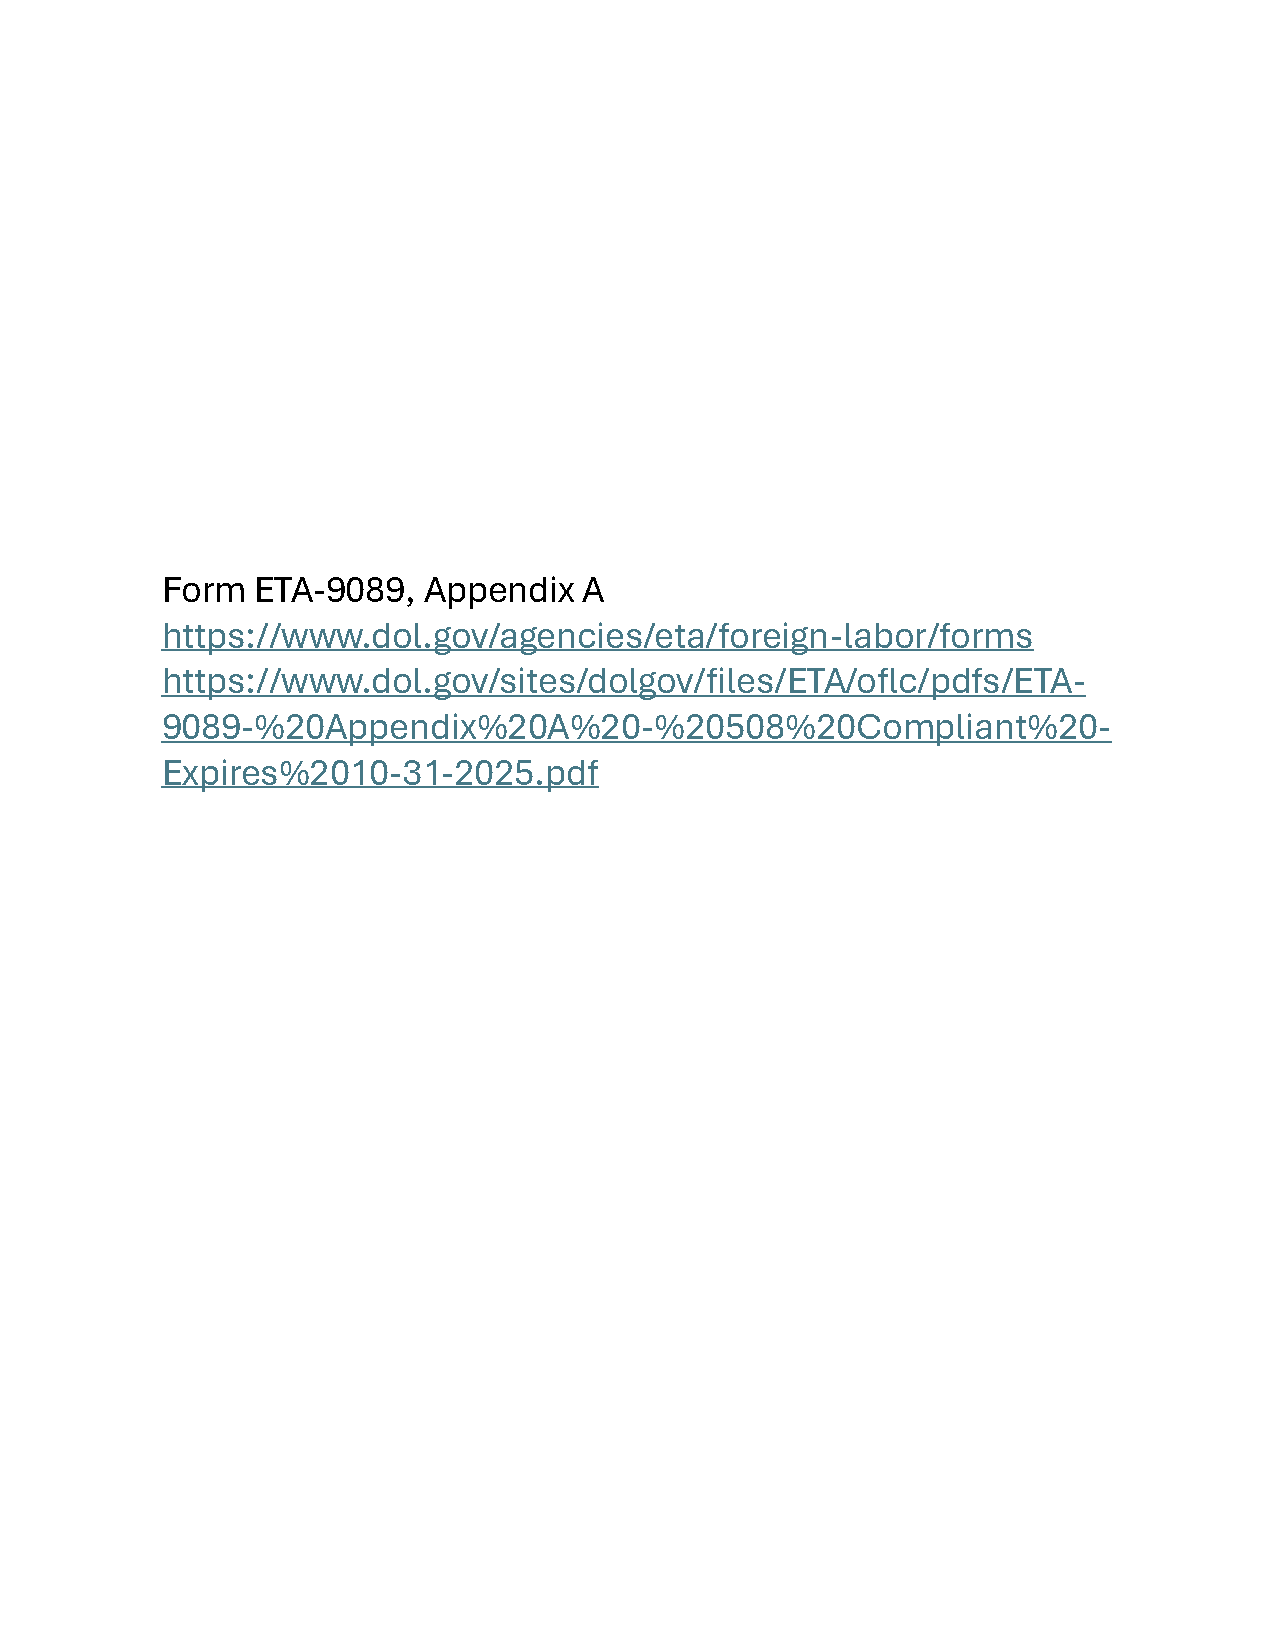
\includepdf[pages=-]{eta-9089-appendix-a.pdf}

\includepdf[pages=-]{eta-9089-final-determination.pdf}

% passport, f1 visa, i-20, i-94

\includepdf[pages=-]{passport.pdf}

\includepdf[pages=-]{visa.pdf}
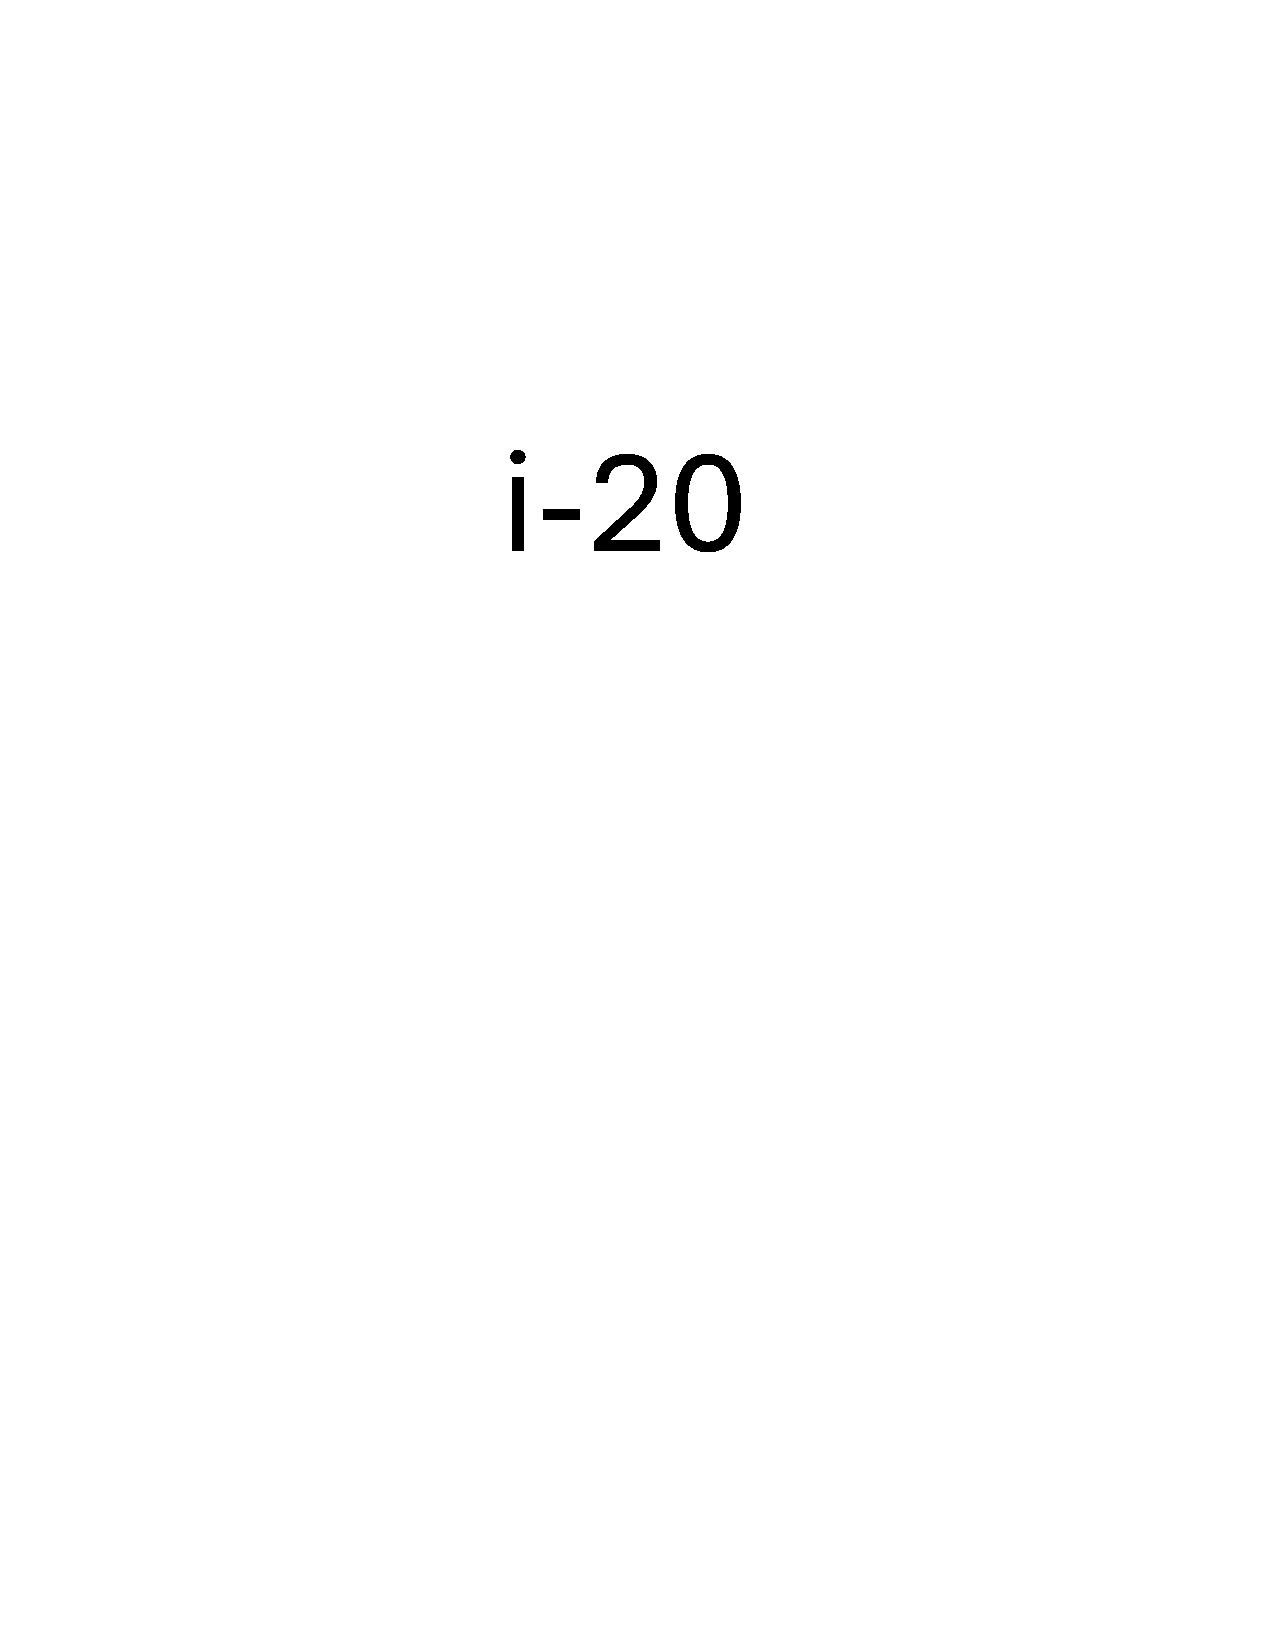
\includepdf[pages=-]{i20.pdf}
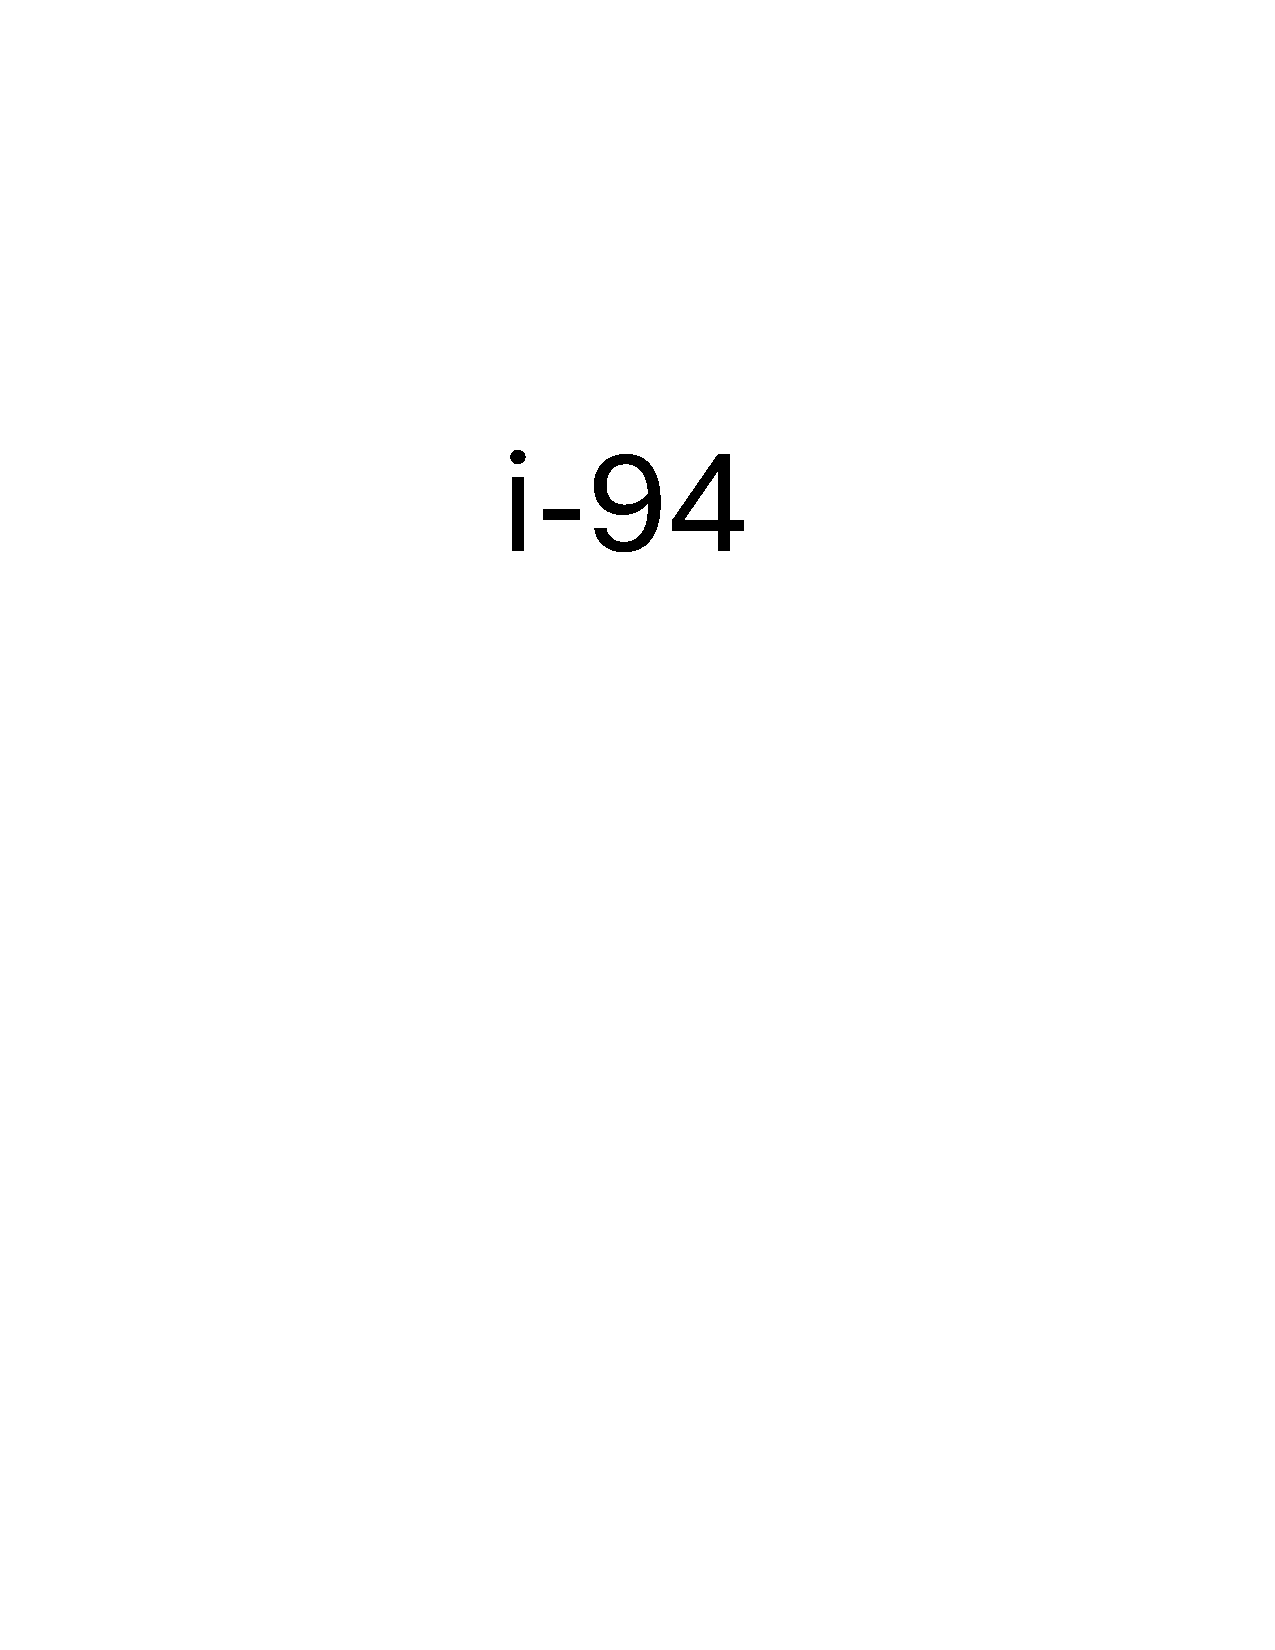
\includepdf[pages=-]{i94.pdf}

\newpage
% set page number from petition letter
\setcounter{page}{1}
% petition letter
U.S. Department of Homeland Security\\
Citizenship and Immigration Services\\
\strut \\
RE: EB-2 Petition for Permanent Residency with request for a National Interest Waiver

\begin{center}
Petitioner/Beneficiary: \quad Mr. \myname \\
Type of Petition: \quad Form I-140\\
Classification Sought: \quad INA §203(b)(2)(B)\\
\strut \\
National Interest Waiver Petition Letter
\end{center}

Dear Immigration Officer:\\
\strut \\
This petition is respectfully submitted in support of Mr. \myname's application for classification as a qualified immigrant under the preference of advanced degree professional/alien of exceptional ability. The evidence submitted herewith will specifically demonstrate that Mr. \myname qualifies for a National Interest Waiver under the standards set by Matter of Dhanasar, 26 I\&N Dec. 884 (AAO 2016).\\
\strut \\
Specifically, the evidence submitted will prove that:\\
1. Mr. \myname is a member of the professions holding an advanced degree;\\
2. Mr. \myname's proposed endeavor has both substantial merit and national importance;\\
3. Mr. \myname is well positioned to advance the proposed endeavor; and\\
4. On balance, it would be beneficial to the United States to waive the
requirements.

\emph{Note that the standard of proof for petitions filed for National
Interest Waiver cases is the ``preponderance of the evidence'' standard.
See Matter of Dhanasar, 26 I\&N Dec. 884, 889 (AAO 2016). Thus, if the
petitioner submits relevant, probative, and credible evidence that leads
USCIS to believe that the claim is ``more likely than not'' or
``probably true,'' the petitioner has satisfied the standard of proof.
Matter of E-M-, 20 I\&N Dec. 77, 79-80 (Comm'r 1989); see also U.S. v.
Cardoza-Fonseca, 480 U.S. 421 (1987) (discussing ``more likely than
not'' as a greater than 50\% chance of an occurrence taking place).}

\newpage

\section{\red{Exhibit Commands Usage Examples (Remove This Section in Final Submission)}}

\vspace{5mm}
\textbf{1. Create an exhibit with an index and label}
\begin{verbatim}
\exhibittext{cv}{1}{CV of Mr. XXXX.}
\end{verbatim}
where "cv" is the label, "1" is the index, and "CV of Mr. XXXX." is the text after the index. It'll be like
\exhibittext{cv}{1}{CV of Mr. XXXX.}.

\vspace{5mm}
\textbf{2. Create an exhibit with an index only}
\begin{verbatim}
\exhibittext{cv-without-lalel}{2}{}.
\end{verbatim}
It'll be like \exhibittext{cv-without-lalel}{2}{}.

\vspace{5mm}
\textbf{3. Refer to an existing exhibit Fully}
\begin{verbatim}
\refexhibit{cv}.
\end{verbatim}
It'll be like \refexhibit{cv}. Note that there are no parentheses here.

\vspace{5mm}
\textbf{4. Refer to an existing exhibit's index}
\begin{verbatim}
\refexhibitnum{cv}.
\end{verbatim}
It'll be like \refexhibitnum{cv}.

%%%%%%%%%%%%%%%%%%%%%%%%%%%%%%%%%%%%%%%%%%%%%%%%%%%%%%%%%
\section{\texorpdfstring{1. MR. \myname IS A MEMBER OF THE PROFESSIONS HOLDING AN ADVANCED DEGREE}{1. MR. \myname IS A MEMBER OF THE PROFESSIONS HOLDING AN ADVANCED DEGREE}}\label{mr.-xxx-is-a-member-of-the-professions-holding-an-advanced-degree}


\exhibittext{ms-in-cs}{3-1}{the Master of Science degree in Computer Science of Mr. First Last.} Moreover, Mr. \myname had a good academic outstanding with a high GPA of 4.0 \exhibittext{ms-in-cs-gpa}{3-2}{the Official Transcript of Mr. First Last.}.


\section{\texorpdfstring{2. MR. \myname\textquotesingle S PROPOSED ENDEAVOR}{2. MR. \myname'S PROPOSED ENDEAVOR}}\label{mr.-xxx-proposed-endeavor}

\section{\texorpdfstring{3. SUBSTANTIAL MERIT AND NATIONAL IMPORTANCE}{3. SUBSTANTIAL MERIT AND NATIONAL IMPORTANCE}}\label{substantial-merit-and-national-importance}

\subsection{\texorpdfstring{3.1. Mr. \myname's Proposed Endeavor Has Substantial Merit}{3.1. Mr. \myname's Proposed Endeavor Has Substantial Merit}}\label{mr.-xxx-proposed-endeavor-has-substantial-merit}

On February 12, 2024, the White House Office of Science and Technology Policy (OSTP) released an updated list of critical and emerging technologies that are potentially significant to U.S. national security. \exhibittext{white-house-list}{9}{Critical and Emerging Technologies List 2024 Update.}

\subsection{\texorpdfstring{3.2. Mr. \myname's Proposed Endeavor Has National Importance}{3.2. Mr. \myname's Proposed Endeavor Has National Importance}}\label{mr.-xxx-proposed-endeavor-has-national-importance}

\section{\texorpdfstring{4. MR. \myname IS WELL POSITIONED TO ADVANCE THE PROPOSED ENDEAVOR}{4. MR. \myname IS WELL POSITIONED TO ADVANCE THE PROPOSED ENDEAVOR }}\label{mr.-xxx-is-well-positioned-to-advance-the-proposed-endeavor}

Dhanasar indicates that the second prong of the analysis must consider whether the petitioner is well positioned to advance the proposed endeavor (Dhanasar, at 890). This multifactorial assessment includes an evaluation of the petitioner's education, skills, knowledge, and record of success in related efforts; a model or plan for future activities; any progress made toward achieving the proposed endeavor; and the interest of potential customers, users, investors, or other relevant entities or individuals (Id.). Importantly, Dhanasar points out the inherent difficulty in "forecasting feasibility or future success", even in the presence of a cogent plan and competent execution;
therefore, petitioners are not required to show that their proposed endeavor is more likely than not to succeed (Id.). \exhibittext{Dhanasar}{22}{the Matter of DHANASAR, Petitioner, 26 I\&N Dec. 884 (AAO 2016)}

\subsection{\texorpdfstring{4.1. Education, Skills, and Knowledge}{4.1. Education, Skills, and Knowledge}}\label{education-skills-and-knowledge}

\subsection{\texorpdfstring{4.2. Mr. \myname has been recognized by the academia}{4.2. Mr. \myname has been recognized by the academia}}\label{mr.-xxx-has-been-recognized-by-the-academia}

\subsection{\texorpdfstring{4.3. Record of Success in Related or Similar Efforts and Interest of Potential Customers, Users, Investors, and Other Relevant Individuals}{4.3. Record of Success in Related or Similar Efforts and Interest of Potential Customers, Users, Investors, and Other Relevant Individuals}}\label{record-of-success-in-related-or-similar-efforts-and-interest-of-potential-customers-users-investors-and-other-relevant-individuals}

\subsubsection{\texorpdfstring{4.3.1. Mr. \myname's research has been published in some of the top conferences and journals in the field}{4.3.1. Mr. \myname's research has been published in some of the top conferences and journals in the field }}\label{mr.-xxx-research-has-been-published-in-some-of-the-top-conferences-and-journals-in-the-field}

\subsubsection{\texorpdfstring{4.3.2. Researchers from around the world have applied upon Mr. \myname\textquotesingle{}s research to further their own research }{ 4.3.2. Researchers from around the world have applied upon Mr. \myname's research to further their own research }}\label{researchers-from-around-the-world-have-applied-upon-mr.-xxx-research-to-further-their-own-research}

\begin{figure}
    \centering
    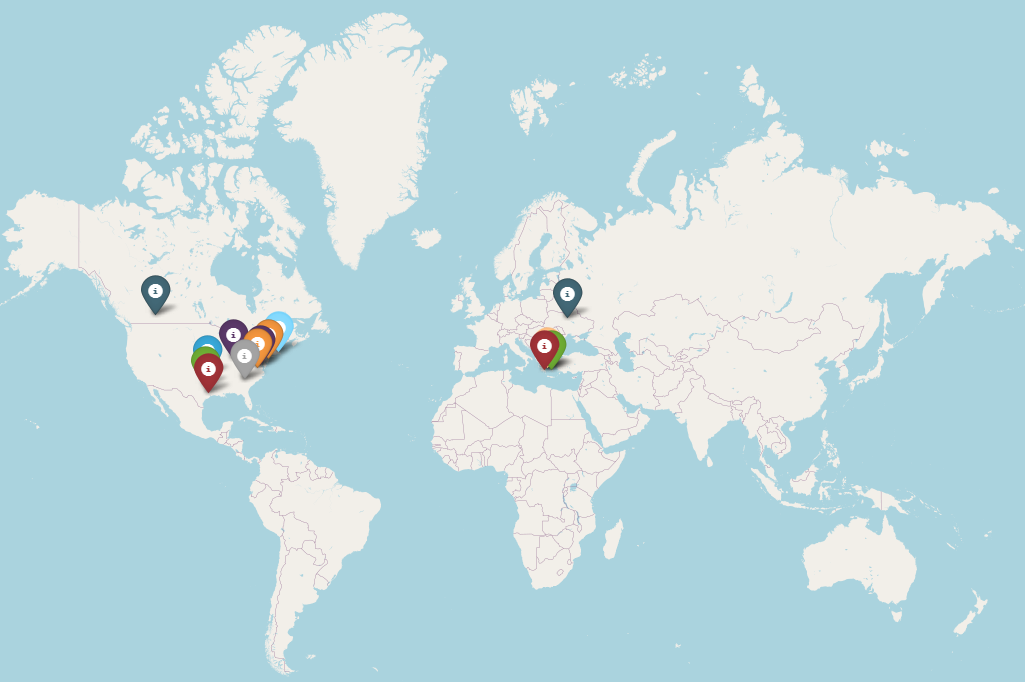
\includegraphics[width=6in,height=3.2in]{map_screenshot.png}
    \caption{The worldwide citation map of Mr. \myname's work.}
    \label{fig:citation_map}
\end{figure}

The citation map can be generated from this Github Repo\footnote{https://github.com/ChenLiu-1996/CitationMap}.

\subsubsection{\texorpdfstring{4.3.3. Mr. \myname served as a reviewer of others\textquotesingle{} research work}{4.3.3. Mr. \myname served as a reviewer of others' research work}}\label{mr.-xxx-served-as-a-reviewer-of-others-research-work}

\subsubsection{\texorpdfstring{4.3.4. Mr. \myname is the awardee of the Fellowships for Graduate Research}{4.3.4. Mr. \myname is the awardee of the Fellowships for Graduate Research}}\label{mr.-xxx-is-the-awardee-of-the-cahmp-summer-fellowships-for-graduate-research}

\subsubsection{\texorpdfstring{4.3.5. Mr. \myname\textquotesingle{}s research is highly novel and influential in the field}{4.3.5. Mr. \myname's is highly novel and influential in the field}}\label{mr.-xxx-research-is-highly-novel-and-influential-in-the-field}

\subsubsection{\texorpdfstring{4.3.6. Mr. \myname\textquotesingle{}s significant original contributions are evident from renowned media}{4.3.6. Mr. \myname's significant original contributions are evident from renowned media}}\label{mr.-xxx-significant-original-contributions-are-evident-from-renowed-media}

\subsubsection{\texorpdfstring{4.3.7. Mr. \myname continuously contributes to U.S. National Science Foundation (NSF) projects}{4.3.7. Mr. \myname continuously contributes to U.S. National Science Foundation (NSF) projects}}\label{mr.-xxx-continuously-contributes-to-us-national-science-foundation-projects}


\subsubsection{\texorpdfstring{4.3.8. Mr. \myname's research and innovations are extensively adopted by users, researchers, and companies}{4.3.8. Mr. \myname's research and innovations are extensively adopted by users, researchers, and companies}}\label{mr.-xxx-research-and-innovations-are-extensively-adopted-by-users-researchers-and-companies}

\subsubsection{\texorpdfstring{4.3.9. Progress toward achieving the proposed endeavor}{4.3.9. Progress toward achieving the proposed endeavor}}\label{progress-toward-achieving-the-proposed-endeavor}

\subsubsection{\texorpdfstring{4.3.10. Plan for future activity in the field}{4.3.10. Plan for future activity in the field}}\label{plan-for-future-activity-in-the-field}

\section{\texorpdfstring{5. ON BALANCE, IT WOULD BE BENEFICIAL TO THE UNITED STATES TO WAIVE THE REQUIREMENTS}{5. ON BALANCE, IT WOULD BE BENEFICIAL TO THE UNITED STATES TO WAIVE THE REQUIREMENTS}}\label{on-balance-it-would-be-beneficial-to-the-united-states-to-waive-the-requirements}

\subsection{\texorpdfstring{5.1. The Significant Benefit of Waiving the Labor Certification Requirement}{5.1. The Significant Benefit of Waiving the Labor Certification Requirement}}


\subsection{\texorpdfstring{5.2. National Interest and Public Benefit}{5.2. National Interest and Public Benefit}}

\subsection{\texorpdfstring{5.3. Economic Impact and Industry Growth}{5.3. Economic Impact and Industry Growth}}

\subsection{\texorpdfstring{5.4. Expertise Beyond Ordinary Training and Value Over Local Workforce}{5.4. Expertise Beyond Ordinary Training and Value Over Local Workforce}}
% ### **Expertise Beyond Ordinary Training and Value Over Local Workforce**


\subsection{\texorpdfstring{5.5. Transdisciplinary Contributions Beyond a Single Employer}{5.5. Transdisciplinary Contributions Beyond a Single Employer}}


\subsection{\texorpdfstring{5.6. Non-Competition with Local Workforce}{5.6. Non-Competition with Local Workforce}}

\subsection{\texorpdfstring{5.7. Reasonability of Waiving PERM and Self-Petition}{5.7. Reasonability of Waiving PERM and Self-Petition}}

\subsection{\texorpdfstring{5.8. Timely Contribution to Emerging Technologies}{5.8. Timely Contribution to Emerging Technologies}}

\subsection{\texorpdfstring{5.9. Unique Expertise and Critical Need}{5.9. Unique Expertise and Critical Need}}

Considering the above factors and the evidence presented therein, Mr.\myname satisfies this prong.

\section{\texorpdfstring{6. CONCLUSION}{6. CONCLUSION}}\label{conclusion}

As the documentary evidence and corroborating testimony from experts in the field establish, Mr.\myname is \emph{\textbf{\ul{a member of the professions holding an advanced degree}}}. He proposes to continue his research on \textbf{SOMETHING}, both of which are included in the \emph{\textbf{\ul{2024 Update of the White House Released Critical and Emerging Technologies List}}}. His endeavor is clearly with \emph{\textbf{\ul{substantial merit}}} and \emph{\textbf{\ul{national importance}}}. Mr. \myname's education, experience, expertise, record of publication and citation, media appearance, industry and academic recognition, and history of successful research in the field all indicate that Mr.\myname is \emph{\textbf{\ul{well positioned to advance the proposed endeavor}}}. These facts establish that it is beneficial to the United States to waive the requirements of a job offer and labor certification.

% index of exhibits
\newpage
\begin{center}
    % \section{}{% create space
    \section{\fontsize{20}{0}\selectfont Index of Exhibits}
    % \section{}{% create space
\end{center}

\section{\red{Exhibit Commands Usage Examples (Remove This Section in Final Submission)}}

\vspace{5mm}
\textbf{1. Create an entry by referring to the index in body.tex}
\begin{verbatim}
\labelexhibit{cv}{CV of Mr. First Last}{cv}
\end{verbatim}
where "cv" is the label in the body.tex (that will be replaced by its index), "CV of Mr. First Last" is the text, and "cv" at the end is the label for this entry. It'll be like

\labelexhibit{cv}{CV of Mr. First Last}{cv}

\vspace{5mm}
\textbf{2. Create an entry by creating a new index}
\begin{verbatim}
\labelexhibit{2}{CV of Mr. First Last}{2}
\end{verbatim}
where "2" is the index showing in "Exhibit 2", "CV of Mr. First Last" is the text, and "2" at the end is the label for this entry (that can be referred to in exhibits.tex). It'll be like

\vspace{5mm}
\labelexhibit{2}{CV of Mr. First Last}{2}

\vspace{5mm}
\red{This is helpful when creating a parent entry to encompass some existing children exhibits in body.tex. For example,}

\begin{verbatim}
\labelexhibit{3}{Master of Science Degree in Computer Science of Mr. First Last}{3}

\labelexhibitsub{ms-in-cs}{Diploma Copy}{ms-in-cs}

\labelexhibitsub{ms-in-cs-gpa}{Official Transcript}{ms-in-cs-gpa}
\end{verbatim} will be like

\labelexhibit{3}{Master of Science Degree in Computer Science of Mr. First Last}{3}

\labelexhibitsub{ms-in-cs}{Diploma Copy}{ms-in-cs}

\labelexhibitsub{ms-in-cs-gpa}{Official Transcript}{ms-in-cs-gpa}

The labels "ms-in-cs" and "ms-in-cs-gpa" are in the body.tex, while "3" is not.

More examples are coming below.
%%%%%%%%%%%%%%%%%%%%%%%%%%%%%%%%%%%%%%%%%%%%%%%%%%%%%%%%%

\labelexhibit{4}{Recommendation Letter from Prof. SOMEONE}{rl-prof-someone}

\red{Note that the following documents are widely in use for the NIW application, so I have included them here.}

\labelexhibit{white-house-list}{Critical and Emerging Technologies List 2024 Update}{white-house-list}

\labelexhibit{Dhanasar}{Matter of DHANASAR, Petitioner, 26 I\&N Dec. 884 (AAO 2016)}{Dhanasar}

\newpage
\newgeometry{top=5cm}

\section{\red{Exhibit Commands Usage Examples (Remove This Section in Final Submission)}}

\vspace{5mm}
\textbf{1. Create a cover page for an exhibit}
\begin{verbatim}
\refexhibitlabel{cv}

\includepdf[pages=-]{cv.pdf}
\end{verbatim}
where "cv" is the label in the index\_of\_exhibits.tex, "cv.pdf" is under exhibits/. It will create a cover page followed by the cv.pdf.

Define pages to be included:

\begin{itemize}
    \item All pages
        \begin{verbatim}
        
\includepdf[pages=-]{cv.pdf}
        \end{verbatim}
    \item One page (1st page)
        \begin{verbatim}
        
\includepdf[pages=1]{cv.pdf}
        \end{verbatim}
    \item Range ([2,3])
        \begin{verbatim}
        
\includepdf[pages=2-3]{cv.pdf}
        \end{verbatim}
    \item Some pages
        \begin{verbatim}
        
\includepdf[pages={1,2}]{cv.pdf}
        \end{verbatim}    
\end{itemize}

\vspace{5mm}
\textbf{2. Create a cover page for a parent exhibit and some child exhibits}
\begin{verbatim}
\refexhibitlabel{3}

\refexhibitsublabel{ms-in-cs}

\refexhibitsublabel{ms-in-cs-gpa}

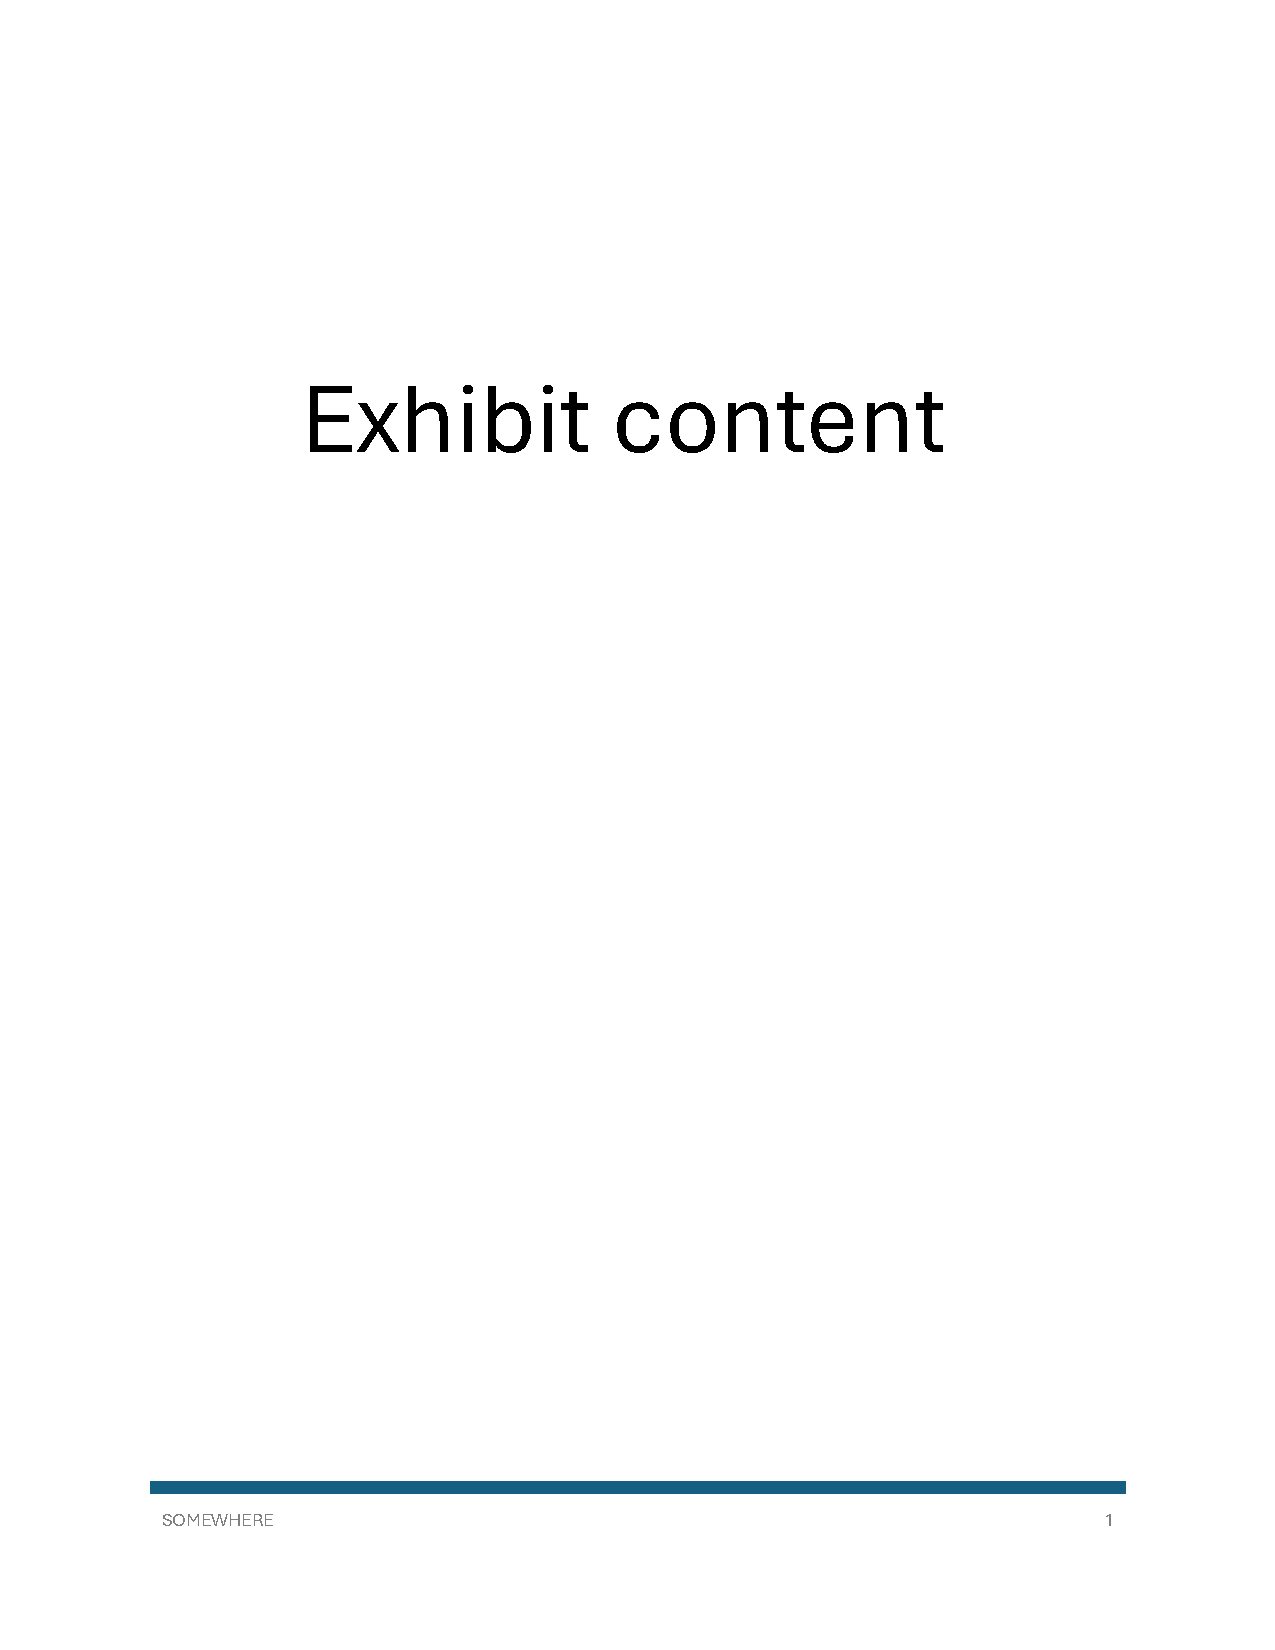
\includepdf[pages=-]{ms-in-cs.pdf}
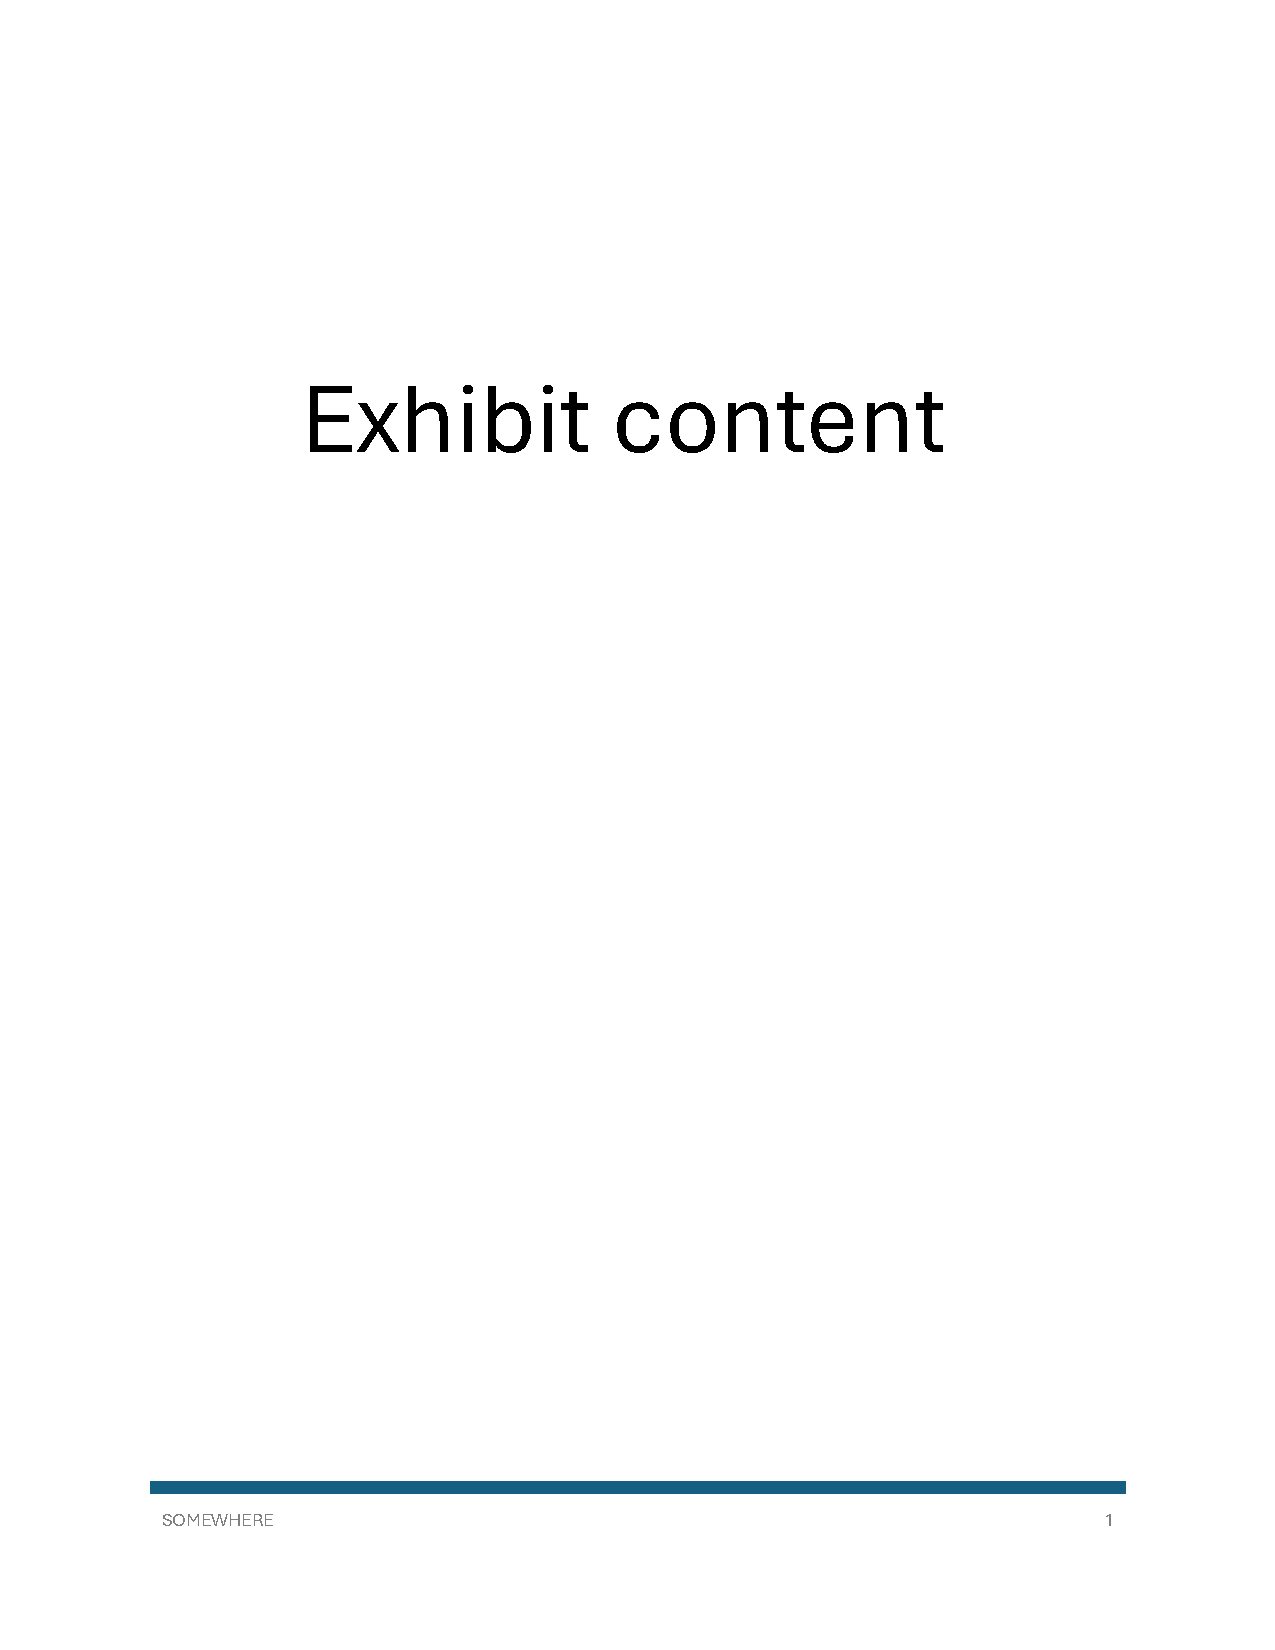
\includepdf[pages=-]{ms-in-cs-gpa.pdf}
\end{verbatim}
where "3", "ms-in-cs", and "ms-in-cs-gpa" are the labels in the index\_of\_exhibits.tex, "ms-in-cs.pdf" and "ms-in-cs-gpa.pdf" are under exhibits/. It will create a cover page followed by the two pdf files. \red{Note the space between `refexhibitlabel` and refexhibitsublabel.}

\refexhibitlabel{3}

\refexhibitsublabel{ms-in-cs}

\refexhibitsublabel{ms-in-cs-gpa}

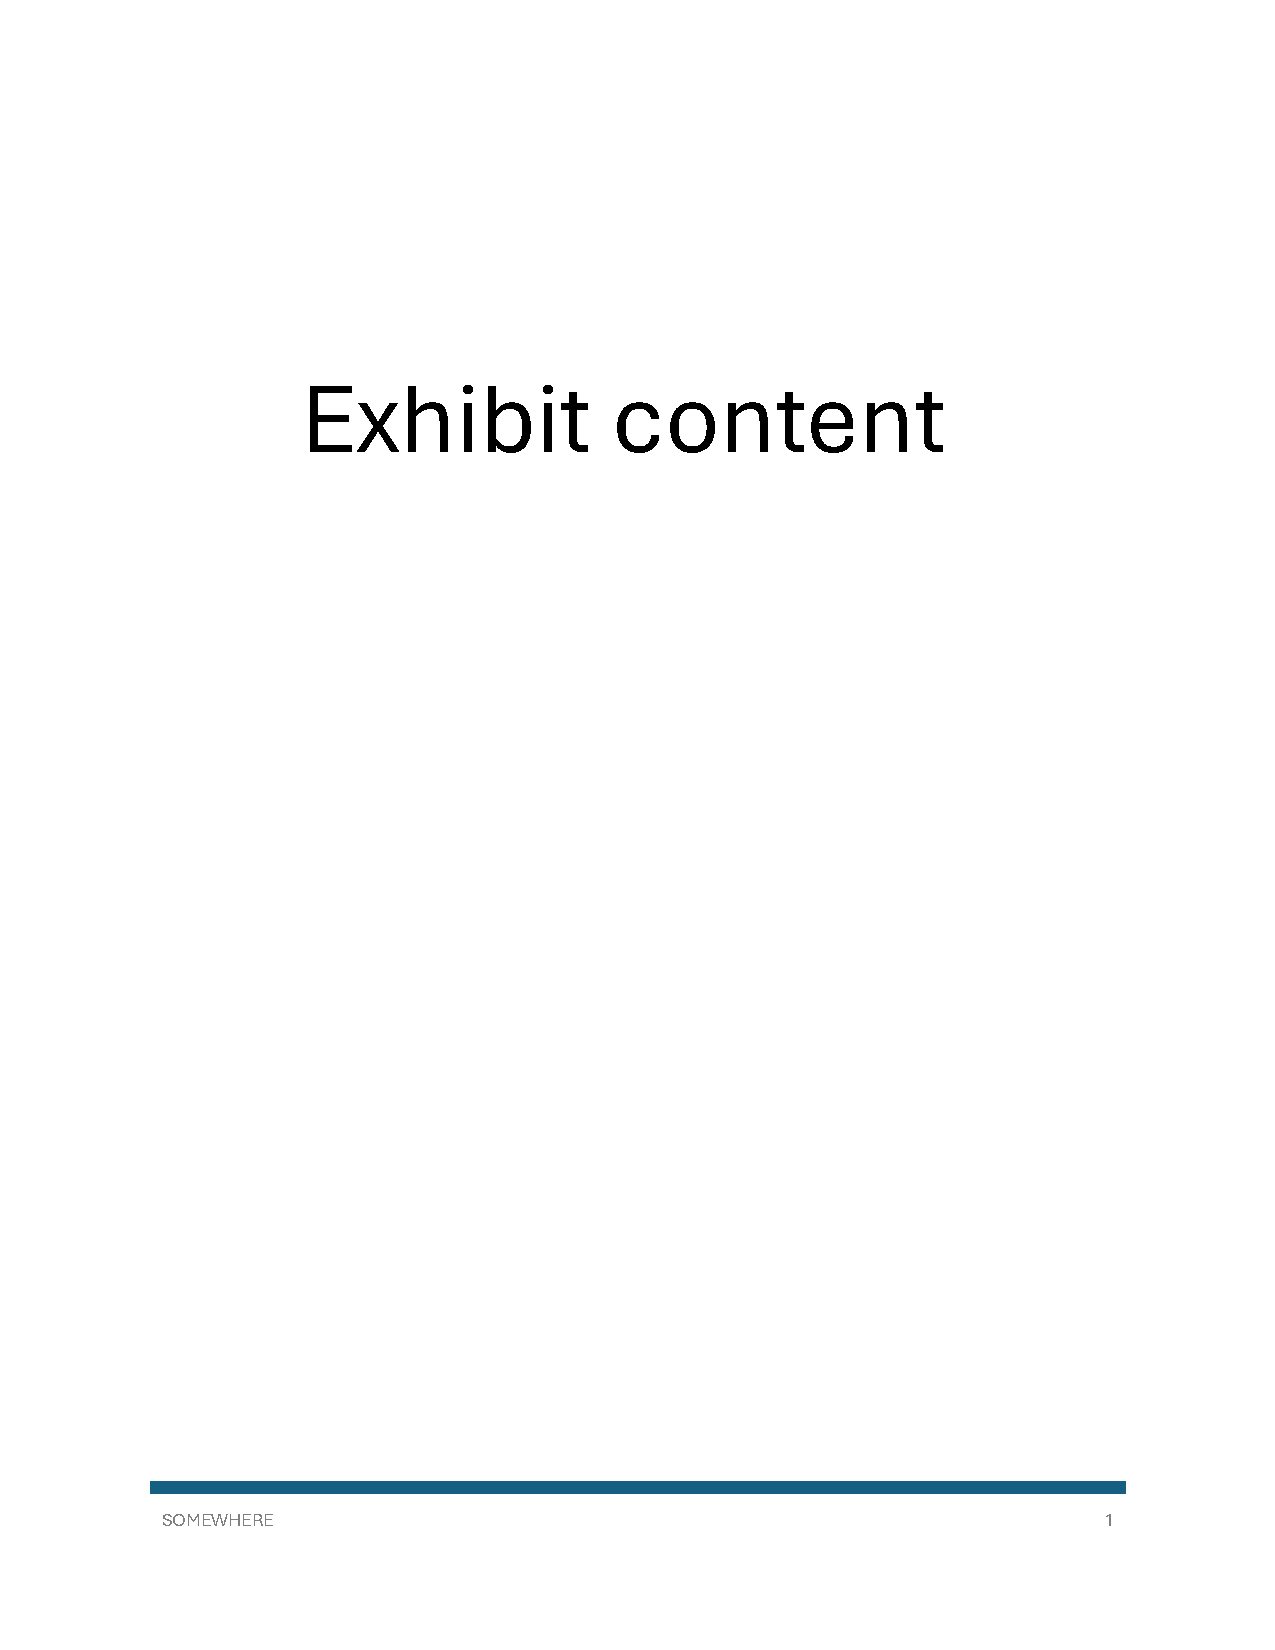
\includepdf[pages=-]{ms-in-cs.pdf}

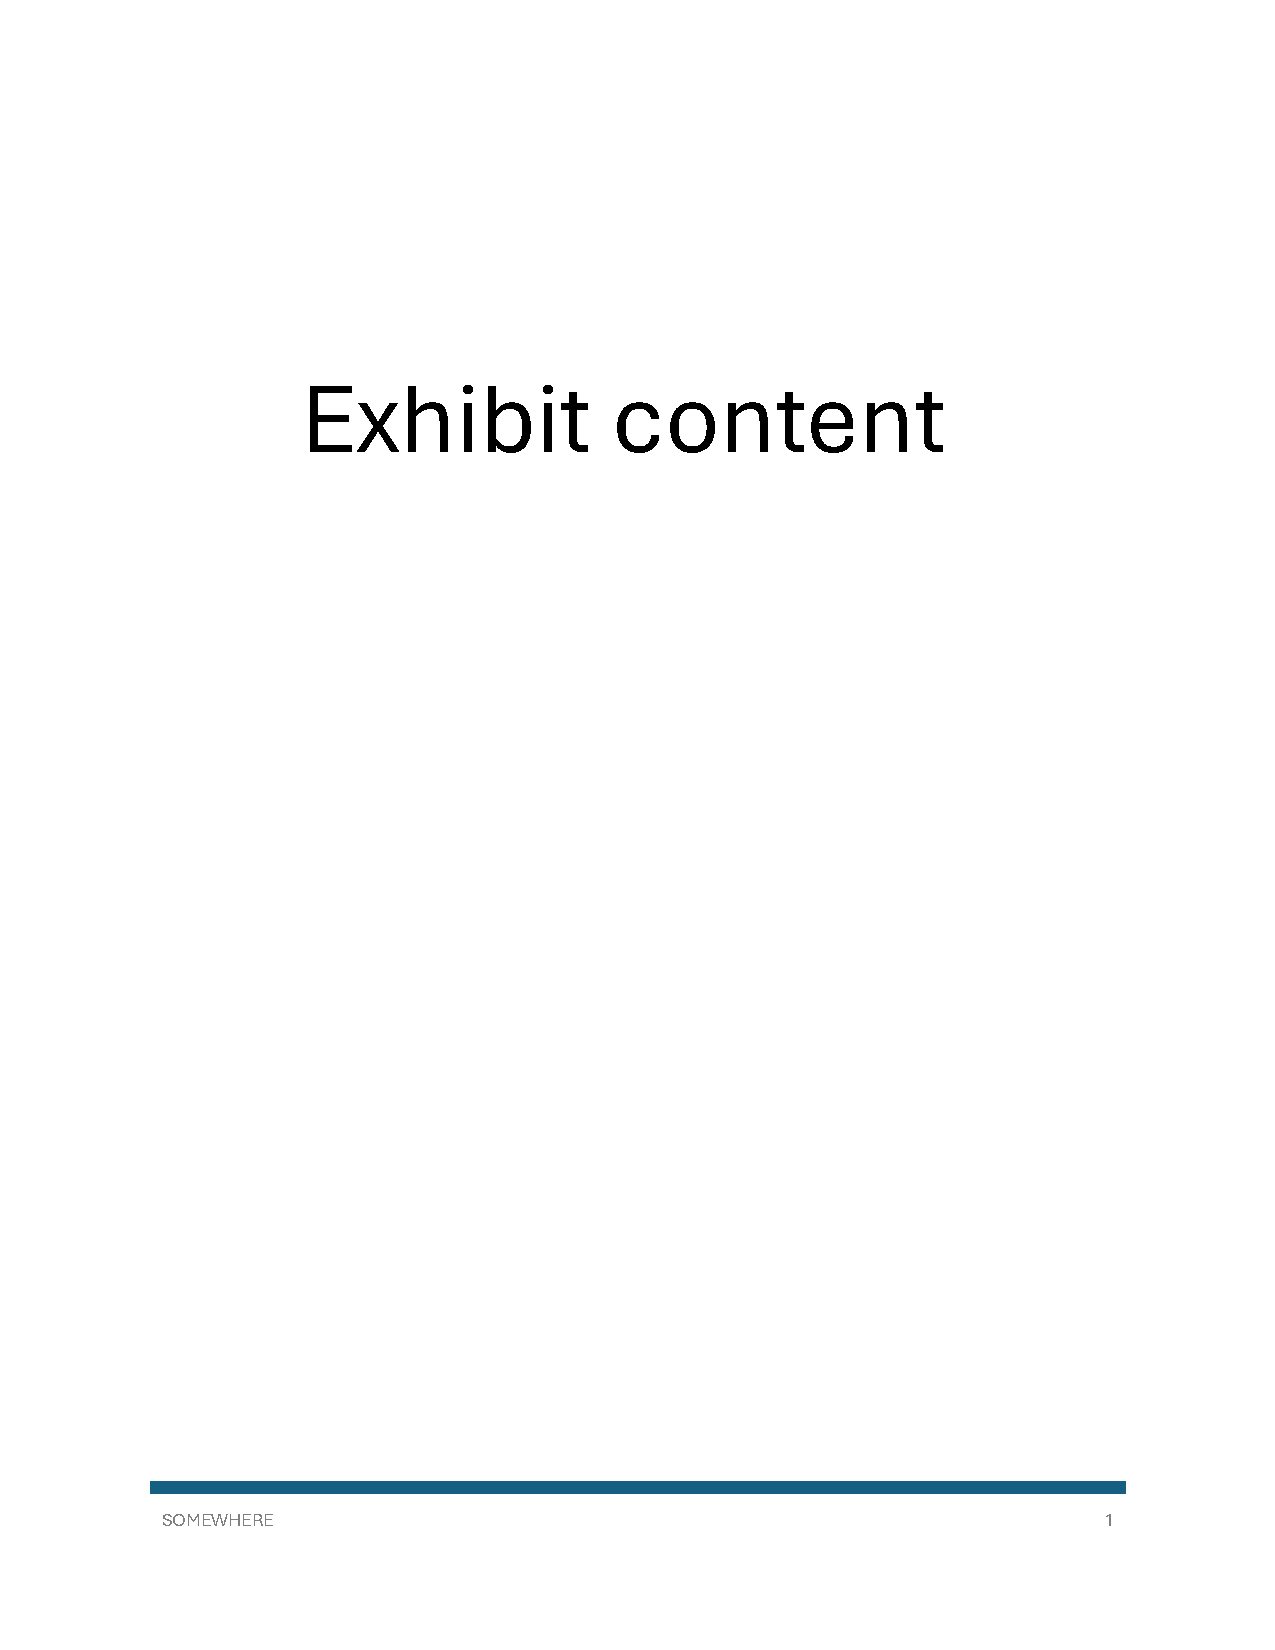
\includepdf[pages=-]{ms-in-cs-gpa.pdf}

More examples are coming below.
%%%%%%%%%%%%%%%%%%%%%%%%%%%%%%%%%%%%%%%%%%%%%%%%%%%%%%%%%
\refexhibitlabel{rl-prof-someone}

\includepdf[pages=-]{recommendation-letter.pdf}

\refexhibitlabel{white-house-list}

\includepdf[pages=-]{white-house-list.pdf}

\refexhibitlabel{Dhanasar}

\includepdf[pages=-]{Dhanasar.pdf}

\restoregeometry

% Good Luck!

\end{document}